\PassOptionsToPackage{unicode=true}{hyperref} % options for packages loaded elsewhere
\PassOptionsToPackage{hyphens}{url}
\documentclass[12pt,ignorenonframetext,aspectratio=169]{beamer}
\IfFileExists{pgfpages.sty}{\usepackage{pgfpages}}{}
\setbeamertemplate{caption}[numbered]
\setbeamertemplate{caption label separator}{: }
\setbeamercolor{caption name}{fg=normal text.fg}
\beamertemplatenavigationsymbolsempty
\usepackage{lmodern}
\usepackage{amssymb}
\usepackage{amsmath}
\usepackage{ifxetex,ifluatex}
\usepackage{fixltx2e} % provides \textsubscript
\ifnum 0\ifxetex 1\fi\ifluatex 1\fi=0 % if pdftex
  \usepackage[T1]{fontenc}
  \usepackage[utf8]{inputenc}
\else % if luatex or xelatex
  \ifxetex
    \usepackage{mathspec}
  \else
    \usepackage{fontspec}
\fi
\defaultfontfeatures{Ligatures=TeX,Scale=MatchLowercase}






%
\fi

  \usetheme[]{iqss}






% use upquote if available, for straight quotes in verbatim environments
\IfFileExists{upquote.sty}{\usepackage{upquote}}{}
% use microtype if available
\IfFileExists{microtype.sty}{%
  \usepackage{microtype}
  \UseMicrotypeSet[protrusion]{basicmath} % disable protrusion for tt fonts
}{}


\newif\ifbibliography


\hypersetup{
      pdftitle={Preparation of financial statements, analysis and agribusiness financing; and investment appraisals},
        pdfauthor={Deependra Dhakal},
          pdfborder={0 0 0},
    breaklinks=true}
%\urlstyle{same}  % Use monospace font for urls







% Prevent slide breaks in the middle of a paragraph:
\widowpenalties 1 10000
\raggedbottom

  \AtBeginPart{
    \let\insertpartnumber\relax
    \let\partname\relax
    \frame{\partpage}
  }
  \AtBeginSection{
    \ifbibliography
    \else
      \let\insertsectionnumber\relax
      \let\sectionname\relax
      \frame{\sectionpage}
    \fi
  }
  \AtBeginSubsection{
    \let\insertsubsectionnumber\relax
    \let\subsectionname\relax
    \frame{\subsectionpage}
  }



\setlength{\parindent}{0pt}
\setlength{\parskip}{6pt plus 2pt minus 1pt}
\setlength{\emergencystretch}{3em}  % prevent overfull lines
\providecommand{\tightlist}{%
  \setlength{\itemsep}{0pt}\setlength{\parskip}{0pt}}

  \setcounter{secnumdepth}{0}


  \usepackage{booktabs}
  \usepackage{longtable}
  \usepackage{emptypage}
  \usepackage{array}
  \usepackage{multirow}
  \usepackage{wrapfig}
  \usepackage{float}
  \usepackage{colortbl}
  \usepackage{pdflscape}
  \usepackage{tabu}
  \usepackage{threeparttable}
  \usepackage{threeparttablex}
  \usepackage[normalem]{ulem}
  \usepackage{rotating}
  \usepackage{makecell}
  \usepackage{xcolor}
  \usepackage{tikz} % required for image opacity change
  \usepackage[absolute,overlay]{textpos} % for text formatting
  \usepackage[utf8]{inputenc}
  \usetikzlibrary{mindmap,arrows,shapes,positioning,shadows,trees}
  \usepackage[skip=2pt]{caption}

  % this font option is amenable for beamer
  \setbeamerfont{caption}{size=\tiny}


%% IQSS overrides
\iqsssectiontitle{Outline}

\AtBeginSection[]{
  \title{\insertsectionhead}
  {
    \definecolor{white}{rgb}{0.776,0.357,0.157}
    \definecolor{iqss@orange}{rgb}{1,1,1}
    \ifnum \insertmainframenumber > \insertframenumber
    \frame{
      \frametitle{\iqsssectiontitleheader}
      \tableofcontents[currentsection]
    }
    \else
    \frame{
      \frametitle{Backup Slides}
      \tableofcontents[sectionstyle=shaded/shaded,subsectionstyle=shaded/shaded/shaded]
    }
    \fi
  }
}

\AtBeginSubsection[]{}

%%


  \title[]{Preparation of financial statements, analysis and
agribusiness financing; and investment appraisals}



  \author[
        Deependra Dhakal
    ]{Deependra Dhakal}

  \institute[
    ]{
    GAASC, Baitadi \and Tribhuwan University
    }

\date[
      \today
  ]{
      \today
        }

\begin{document}

% Hide progress bar and footline on titlepage
  \begin{frame}[plain]
  \titlepage
  \end{frame}



\hypertarget{financial-statements-preparation-and-analysis}{%
\section{Financial statements -- Preparation and
analysis}\label{financial-statements-preparation-and-analysis}}

\begin{frame}{Background}
\protect\hypertarget{background}{}
\begin{itemize}
\tightlist
\item
  Financial statement shows the financial position and performance of a
  business
\item
  Thoroughly understanding your business' financial performance is
  critical for success in today's increasingly competitive agricultural
  environment.
\item
  Successful managers use financial statements in combination with
  production records to identify strengths and weaknesses in their
  operation.
\item
  Financial statements include the balance sheet, income statement,
  statement of owner equity, statement of cash flows.
\end{itemize}
\end{frame}

\begin{frame}{Balance sheet/Net worth statement}
\protect\hypertarget{balance-sheetnet-worth-statement}{}
\begin{itemize}
\tightlist
\item
  The balance sheet, also called net worth or financial statement, is a
  summary of assets and liabilities of a business together with the
  statement of the owners' equity or net worth.
\item
  This is a listing of all assets and liabilities of a farm at certain
  point of time.
\item
  This reports the financial strength and progress of the business.
\item
  The term balance here implies that the value of the assets must be
  equal to the value fo liabilities plus owner's equity or net worth.
\end{itemize}
\end{frame}

\begin{frame}{Characteristics of a balance sheet}
\protect\hypertarget{characteristics-of-a-balance-sheet}{}
\footnotesize

\begin{itemize}
\tightlist
\item
  Pertains to specific point of time. i.e.~24th January, 1994.
\item
  It characterizes the three essential components. i.e.~assets,
  liabilities and net worth/owner's equity.
\item
  It includes either owned or owed items and does not provide an
  accurate measure of total assets controlled, since many assets used in
  the production may be rented in.
\item
  The balance sheet can be prepared for a farm business or farm
  operator's family. The assets are presented in order of payments or
  liquidity. Moreover the liabilities are written on left side while
  assets towards right side.
\item
  The balance sheet does not indicate the progress or deterioration if
  the farm business, unless drawn overtime and net worth is compared.
\item
  The balance sheet can be constructed on a cost basis/book value
  (purchase price or original cost minus depreciation) or current market
  value basis.
\item
  Sometimes the physical data is also given to see the changes in
  inventory value, changes in unit prices or changes in both inventory
  and prices.
\item
  Net worth is placed towards liabilities' side as the owners like
  creditor has claim against the business for the assets equal to net
  worth. In fact it is the liability of the business which owes that
  amount to the owner. But net deficit is placed on the asset side to
  show the shortage of assets.
\end{itemize}
\end{frame}

\begin{frame}{}
\protect\hypertarget{section}{}
\textbf{Liabilities}: It represents an amount which is owned to others
whether payable in cash, kind or services.

\textbf{Current liability}: These are the debts payable within the
operating year, normally 12 month. e.g., crop loan.

\textbf{Long term liabilities}: There are the obligations associated
with the intermediate and long term assets, respectively. Once should
consider outstanding principle which is due beyond 12 months as
intermediate or long term liabilities. Medium term loans or liabilities
are those whose maturity between 1 and 7 years while long term loans or
liabilities possess maturity more than 7 years.

\textbf{Contingent liabilities}: These become due under specific
circumstances, such as capital gain taxes. Such taxes become due only
when the capital asset is sold. Such liabilities are only accounted for
if the balance sheet is prepared on the market value basis.
\end{frame}

\begin{frame}{}
\protect\hypertarget{section-1}{}
\begin{itemize}
\tightlist
\item
  An asset is essentially a resource held by the business. The
  characteristics of an asset are:

  \begin{enumerate}
  \tightlist
  \item
    A probable future benefit must exist.
  \item
    The business must have an exclusive rights to control the benefit.
  \item
    The benefit must arise from some past transaction or event.
  \item
    The asset must be capable of measurement in monetary terms.
  \end{enumerate}
\end{itemize}
\end{frame}

\begin{frame}{}
\protect\hypertarget{section-2}{}
\begin{itemize}
\tightlist
\item
  Assets can be further classified as follows in sequence of their
  liquidity,
\end{itemize}

\textbf{Current assets}: These are consumed within the single year and
can be converted into cash without disrupting the farm business (sale of
land disrupts the farm business)

\textbf{Medium term assets}: These assets cannot be converted or sold
for cash in short period of time e.g.~milch and draught animals, small
equipment etc. These assets are not consumed within the year and
continue to give returns beyond one year.

\textbf{Long term/fixed assets}: These are also part of production plan
but are of permanent nature. Farm real state represents the major long
term asset on the balance sheet for most farm operators.
\end{frame}

\begin{frame}{Example}
\protect\hypertarget{example}{}
\begin{columns}

\column{0.4\textwidth}
\scalebox{0.60}{\begin{minipage}{1.2\textwidth}
\begin{itemize}
\item Net worth or equity or net assets or capital of a company/farm is calculated by calculating the difference between the Total Assets and the Total Liabilities.
\item An example Net worth statement of MudnBrick Commercial Vegetable and Livestock Farm is presented in Table \ref{tab:net-worth-state}.
\end{itemize}
\end{minipage}}

\column{0.8\textwidth}
\scalebox{0.6}{\begin{minipage}{1.2\textwidth}

\begin{table}[H]

\caption{\label{tab:net-worth-state}Net worth statement}
\centering
\fontsize{8}{10}\selectfont
\begin{tabular}[t]{llll}
\toprule
\multicolumn{4}{c}{\textbf{MudnBrick Commercial Vegetable and Livestock Farm}} \\
\cmidrule(l{3pt}r{3pt}){1-4}
\multicolumn{4}{c}{\em{Financial condition as of 2011-11-11}} \\
\cmidrule(l{3pt}r{3pt}){1-4}
\multicolumn{4}{c}{\textbf{Net Worth Statement}} \\
\cmidrule(l{3pt}r{3pt}){1-4}
 &  &  \vphantom{1} & \\
\midrule
\rowcolor{gray!6}  \multicolumn{1}{c}{\textbf{Assets}} & \multicolumn{1}{c}{\textbf{Market value}} & \multicolumn{1}{c}{\textbf{Liabilities}} & \multicolumn{1}{c}{\textbf{Amount}}\\
\multicolumn{1}{c}{\textbf{Current}} & \multicolumn{1}{c}{\textbf{}} & \multicolumn{1}{c}{\textbf{Short-term}} & \multicolumn{1}{c}{\textbf{}}\\
\rowcolor{gray!6}  Cash in hand & 450 & Accounts payable & 14000\\
Checking/savings & 500 & Unpaid taxes and interest & 35000\\
\rowcolor{gray!6}  Inventory & 9000 & Veterinary fees & 0\\
\addlinespace
Accounts receivables & 8000 & Other short term loan & 9000\\
\rowcolor{gray!6}  Cash at bank & 5000 &  & \\
\multicolumn{1}{c}{\textbf{Current total}} & \multicolumn{1}{c}{\textbf{22950}} & \multicolumn{1}{c}{\textbf{Short-term total}} & \multicolumn{1}{c}{\textbf{58000}}\\
\rowcolor{gray!6}  \multicolumn{1}{c}{\textbf{Non-current/Fixed}} & \multicolumn{1}{c}{\textbf{}} & \multicolumn{1}{c}{\textbf{Long term}} & \multicolumn{1}{c}{\textbf{}}\\
Farm real estate & 150000 & Farm real estate & 90000\\
\addlinespace
\rowcolor{gray!6}  Tractor & 1500 & Automobile loan & 20000\\
Farm equipments & 13000 & Building depreciation & 400\\
\rowcolor{gray!6}  Personal property & 5000 & Farm animal purchase loan & 12000\\
Farm animals and livestocks & 14000 &  & \\
\rowcolor{gray!6}  \multicolumn{1}{c}{\textbf{Non-current/Fixed total}} & \multicolumn{1}{c}{\textbf{183500}} & \multicolumn{1}{c}{\textbf{Long term total}} & \multicolumn{1}{c}{\textbf{122400}}\\
\addlinespace
Investment/Long term &  &  \vphantom{1} & \\
\rowcolor{gray!6}  Stocks & 1000 &  & \\
Bonds & 100 &  & \\
\rowcolor{gray!6}  Goodwill & 5000 &  & \\
Cash value of livestock insurance & 4000 &  & \\
\addlinespace
\rowcolor{gray!6}  \multicolumn{1}{c}{\textbf{Investment/Long term total}} & \multicolumn{1}{c}{\textbf{10100}} & \multicolumn{1}{c}{\textbf{}} & \multicolumn{1}{c}{\textbf{}}\\
 &  &  & \\
\rowcolor{gray!6}  \multicolumn{1}{c}{\textbf{Total assets}} & \multicolumn{1}{c}{\textbf{216550}} & \multicolumn{1}{c}{\textbf{Total liabilities}} & \multicolumn{1}{c}{\textbf{180400}}\\
\multicolumn{1}{c}{\textbf{Net worth}} & \multicolumn{1}{c}{\textbf{36150}} & \multicolumn{1}{c}{\textbf{}} & \multicolumn{1}{c}{\textbf{}}\\
\bottomrule
\end{tabular}
\end{table}

\end{minipage}}
\end{columns}
\end{frame}

\begin{frame}{Farm income statement/Profit and loss account}
\protect\hypertarget{farm-income-statementprofit-and-loss-account}{}
\footnotesize

\begin{itemize}
\tightlist
\item
  Balance sheet shows only the amount of wealth held by a business at
  one moment in time.
\item
  Profit generated during a period is a main concern of many users of
  financial statements.
\item
  P\&L statement provides a picture of profitability of the farm.

  \begin{itemize}
  \tightlist
  \item
    How much wealth (that is, profit) was generated, or lost, by the
    business over that period?
  \end{itemize}
\item
  Profit (loss) is defined as the increase (decrease) in wealth arising
  from trading activities.
\item
  This is more accurately done using an accrual statement, which further
  accounts for inventory, accounts payable, and receivables, as well as
  depreciation expense.
\item
  The difference between the total revenue and total expenses will
  represent either profit (if revenue exceeds expenses) or loss (if
  expenses exceed revenue).
\item
  The period over which profit or loss is normally measured is usually
  known as the ``accounting period'', or ``financial period''.
\end{itemize}
\end{frame}

\begin{frame}{}
\protect\hypertarget{section-3}{}
\begin{itemize}
\tightlist
\item
  Measuring profit is done after first identifying total revenue
  generated during a particular period of the business.
\item
  \textbf{Revenue} is simply a measure of the inflow of economic
  benefits arising from the ordinary activities of a business.
\item
  These benefits, which accrue to the owners, will result in either an
  increase in assets (such as cash or amounts owed to the business by
  its customers) or a decrease in liabilities. Some examples of the
  different forms that revenue can take are as follows:

  \begin{itemize}
  \tightlist
  \item
    sales of goods/crops (for example, of a producer)
  \item
    fees for services (for example, of a packaging)
  \item
    subscriptions (for example, of a cooperative)
  \item
    interest received (for example, of an investment fund).
  \end{itemize}
\end{itemize}
\end{frame}

\begin{frame}{}
\protect\hypertarget{section-4}{}
\footnotesize

\begin{itemize}
\tightlist
\item
  The total expenses relating to each period must also be identified.
\item
  \textbf{Expense} represents the outflow of economic benefits arising
  from the ordinary activities of a business. This loss of benefits will
  result in either a decrease in assets (such as cash) or an increase in
  liabilities (such as amounts owed to suppliers). Expenses are incurred
  in the process of generating revenue, or attempting to generate it.
  Examples of some of the more common types of expenses are:

  \begin{itemize}
  \tightlist
  \item
    the cost of buying goods that are subsequently sold - known as cost
    of sales or cost of goods sold
  \item
    salaries and wages
  \item
    rent and rates
  \item
    farm machinery and vehicle running expenses
  \item
    insurances
  \item
    printing and stationery
  \item
    energy expenses (heat and light)
  \item
    telephone and postage.
  \end{itemize}
\end{itemize}
\end{frame}

\begin{frame}{Example}
\protect\hypertarget{example-1}{}
\begin{table}[H]

\caption{\label{tab:cost-return-an}Income statement}
\fontsize{6}{8}\selectfont
\begin{tabular}[t]{rll}
\toprule
\multicolumn{3}{c}{\textbf{Income statement}} \\
\cmidrule(l{3pt}r{3pt}){1-3}
\em{\textbf{}} & \em{\textbf{Particulars}} & \em{\textbf{Amount (Rs./ropani/annum)}}\\
\midrule
\rowcolor{gray!6}  1 & Sales revenue of vegetables and dairy product & \textcolor[HTML]{BBDF27}{\textbf{55000}}\\
2 & Less cost of sales (Marketing, transport, etc.) & \textcolor[HTML]{46065A}{\textbf{1200}}\\
\rowcolor{gray!6}  \multicolumn{1}{c}{\textbf{}} & \multicolumn{1}{c}{\textbf{Gross profit}} & \multicolumn{1}{c}{\textbf{\textcolor[HTML]{ADDC30}{\textbf{53800}}}}\\
1 & Less salaries and wages payment of farm keepers & \textcolor[HTML]{2D708E}{\textbf{22514}}\\
\rowcolor{gray!6}  2 & Less heat and light cost & \textcolor[HTML]{46065A}{\textbf{1200}}\\
\addlinespace
3 & Less insurance & \textcolor[HTML]{481E70}{\textbf{5331.6}}\\
\rowcolor{gray!6}  4 & Less motor vehicle running expenses & \textcolor[HTML]{460B5E}{\textbf{2200}}\\
5 & Less depreciation - fixtures and fittings & \textcolor[HTML]{450457}{\textbf{800}}\\
\rowcolor{gray!6}  6 & Less depreciation - Vehicles & \textcolor[HTML]{440154}{\textbf{400}}\\
\multicolumn{1}{c}{\textbf{}} & \multicolumn{1}{c}{\textbf{Operating profit}} & \multicolumn{1}{c}{\textbf{\textcolor[HTML]{2F6B8E}{\textbf{21354.4}}}}\\
\addlinespace
\rowcolor{gray!6}  1 & Interest received from investments & \textcolor[HTML]{460A5D}{\textbf{2000}}\\
2 & Less interest on borrowings & \textcolor[HTML]{450457}{\textbf{900}}\\
\rowcolor{gray!6}  \multicolumn{1}{c}{\textbf{}} & \multicolumn{1}{c}{\textbf{Profit for the period}} & \multicolumn{1}{c}{\textbf{\textcolor[HTML]{2D708E}{\textbf{22454.4}}}}\\
\bottomrule
\end{tabular}
\end{table}
\end{frame}

\begin{frame}{Statement of cash flows}
\protect\hypertarget{statement-of-cash-flows}{}
\begin{itemize}
\tightlist
\item
  It shows possible shortfalls in cash and thus allows for corrective
  measures.
\item
  Unfortunately, this is usually the most neglected management tool.
\item
  The statement of cash flows, as the name implies, is a summary of the
  actual cash inflows and cash outflows experienced by a business during
  an accounting period.
\item
  Table \ref{fig:cash-flow-statement} is I. M. Farmer's Statement of
  Cash Flows for the year ending December 31, 2017.
\item
  This statement is organized around five broad categories:

  \begin{itemize}
  \tightlist
  \item
    operating: cash farm income and expenses;
  \item
    investing: capital assets;
  \item
    financing: loans and repayments;
  \item
    nonfarm items; and
  \item
    balancing section for cash on hand.
  \end{itemize}
\item
  Noncash transactions, even though they affect farm profit or net
  worth, are not included in a statement of cash flows.
\end{itemize}
\end{frame}

\begin{frame}{Example}
\protect\hypertarget{example-2}{}
\begin{figure}

{\centering 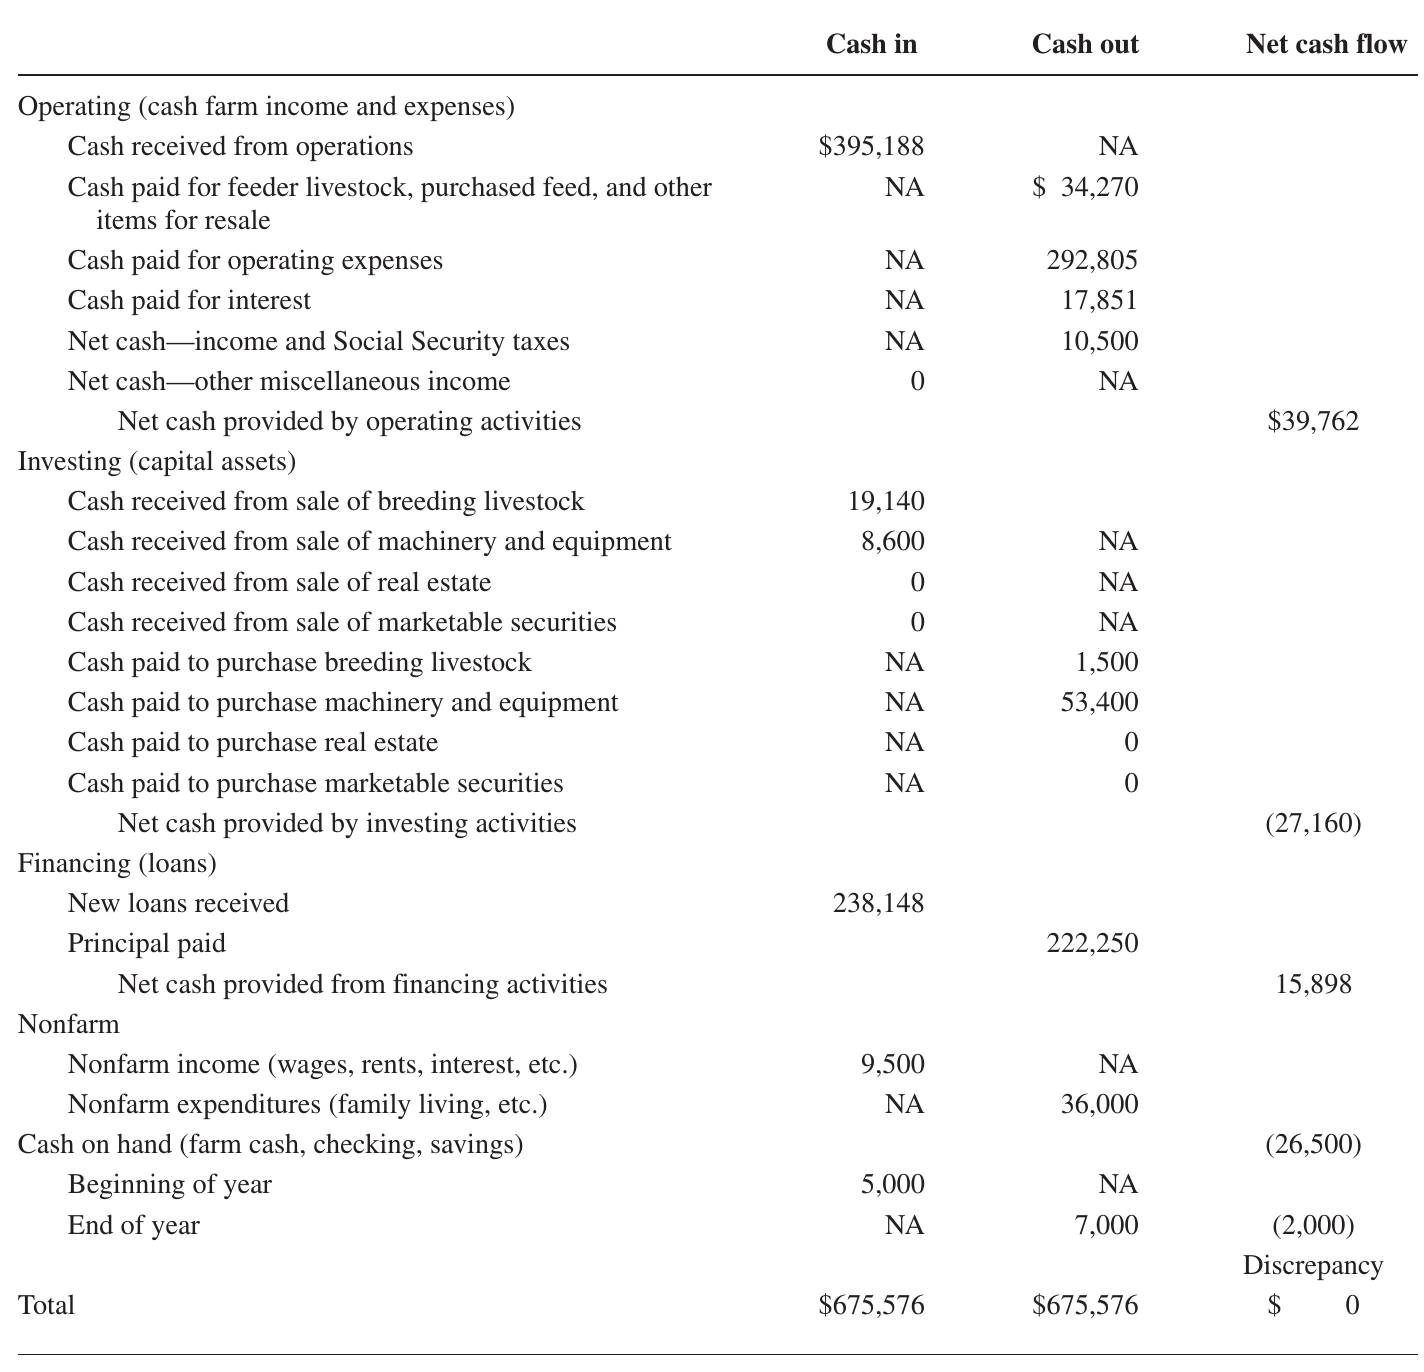
\includegraphics[width=.8\textwidth]{./figs/cash_flow_statement} 

}

\caption{Statement of cash flow of I.M Farmer's for the year ending December 31, 2017}\label{fig:cash-flow-statement}
\end{figure}
\end{frame}

\hypertarget{investment-appraisal-criteria}{%
\section{Investment appraisal
criteria}\label{investment-appraisal-criteria}}

\begin{frame}{Background}
\protect\hypertarget{background-1}{}
\begin{itemize}
\tightlist
\item
  Key steps involved in determining whether a project is worthwhile or
  not are:

  \begin{itemize}
  \tightlist
  \item
    Calculate the costs and benefit of the project
  \item
    Assess the riskiness of the project
  \item
    Calculate the cost of capital
  \item
    Compute the criteria of merit and judge whether the project is good
    or bad
  \end{itemize}
\end{itemize}
\end{frame}

\begin{frame}{Principle of time value of money}
\protect\hypertarget{principle-of-time-value-of-money}{}
\begin{itemize}
\tightlist
\item
  It refers to the purchasing power of money associated with time factor
\item
  Increase in the purchasing power of money as compared to future period
  of time in current scenario.
\end{itemize}

\begin{enumerate}
\tightlist
\item
  Compounding (Future value of present money)
\item
  Discounting (Present value of future money)
\end{enumerate}
\end{frame}

\begin{frame}{}
\protect\hypertarget{section-5}{}
\begin{itemize}
\tightlist
\item
  There are many criteria that have been suggested by economists,
  accountants, and others to judge the worthwhileness of capital
  projects
\item
  Some are general and applicable to a wide range of investments, others
  are specialized and suitable for certain types of investments and
  industries.
\item
  The important investment criteria, classified into two broad
  categories-discounting criteria and non-discounting criteria.
\end{itemize}
\end{frame}

\begin{frame}{}
\protect\hypertarget{section-6}{}
\textbf{Discounting criteria}

\begin{itemize}
\tightlist
\item
  This method takes into account of the time value of money (Discounting
  means the calculation of present value of future worth)
\item
  There are mainly three popular methods used for evaluating alternative
  investment activities: NPV, BC ratio, IRR
\end{itemize}

\textbf{Non discounting criteria}

\begin{itemize}
\tightlist
\item
  This method does not take into account the time value of money and is
  not that much popular.
\item
  Payback period, Accounting rate of return, proceed per unit of outlay,
  simple rate of return
\end{itemize}
\end{frame}

\hypertarget{discounting-criteria}{%
\section{Discounting criteria}\label{discounting-criteria}}

\begin{frame}{Net present value/worth (NPV)}
\protect\hypertarget{net-present-valueworth-npv}{}
\begin{itemize}
\tightlist
\item
  NPV of a project is the sum of the present value of all the cash
  flows-positive as well as negative that are expected to occur over the
  life of the project
\item
  NPV of a project is the present worth of the benefit less the present
  worth of the costs.
\item
  It is simply the present worth/value of the incremental net benefit or
  incremental cash flow stream.
\item
  Mathematically,
\end{itemize}

\begin{columns}
\footnotesize

\column{0.6\textwidth}
\scalebox{0.60}{\begin{minipage}{1.2\textwidth}

$$
NPV = \frac{CF_0}{(1 + r)^0} + \frac{CF_1}{(1 + r)^1} + \frac{CF_2}{(1 + r)^2} + \ldots + \frac{CF_n}{(1 + r)^n} = \sum_{n = i}^n{\frac{CF_n}{(1 + r)^n}}
$$

Where, 

CF = incremental benefit ($\textrm{Benefit stream}- \textrm{Cost stream}$), 

n = number of years, 

r = rate of interest
\end{minipage}}

\column{0.4\textwidth}

Decision criteria

\begin{itemize}
\item NPV > 0 $\longrightarrow$ Project accepted
\item NPV = 0 $\longrightarrow$ Indifferent in decision making
\item NPV < 0 $\longrightarrow$ Project rejected
\end{itemize}

\end{columns}
\end{frame}

\begin{frame}{Benefit cost ratio}
\protect\hypertarget{benefit-cost-ratio}{}
\begin{itemize}
\tightlist
\item
  BC ratio is the oldest method among all discounted measures of project
  evaluation.
\item
  It is the ratio of present worth of benefit stream divided by the
  present worth of cost stream.
\end{itemize}

\begin{columns}

\column{0.5\textwidth}

$$
\large
\textrm{BC ratio} = \frac{\sum_{t = 1}^n{\frac{B_t}{(1 + r)^t}}}{\sum_{t = 1}^n{\frac{C_t}{(1 + r)^t}}}
$$

\column{0.5\textwidth}

Decision criteria

\begin{itemize}
\item BC ratio > 1 $\longrightarrow$ Project accepted
\item BC ratio = 1 $\longrightarrow$ Indifferent in decision making
\item BC ratio < 1 $\longrightarrow$ Project rejected
\end{itemize}

\end{columns}
\end{frame}

\begin{frame}{Internal rate of return}
\protect\hypertarget{internal-rate-of-return}{}
\footnotesize

\begin{itemize}
\tightlist
\item
  It is discount rate which makes its NPV equal to zero
\item
  In another word, it is the discount rate which equates the present
  value of future cash flows with the initial investment
\item
  Therefore, in IRR method the interest rate that equates the present
  value of the future cash earnings with initial investment outlay is
  calculated
\item
  If IRR is used in financial analysis, it is named as financial rate of
  return and in economic analysis, it is called economic rate of return
\item
  It is actually the earning rate of the project under evaluation
\item
  Mathematically,
\end{itemize}

\begin{columns}

\column{0.5\textwidth}
\scalebox{0.60}{\begin{minipage}{1.2\textwidth}

$$
\textrm{IRR} = LDR + D\times \frac{\textrm{NPV at LDR}}{|\textrm{Sum of NPV at TDR}|}
$$
\end{minipage}}

\column{0.5\textwidth}

Decision criteria

\begin{itemize}
\item In case of single project, accept the project when IRR is greater than opportunity cost of capital; i.e. market interest rate is generally between 14-19\%.
\item In case of two mutually exclusive projects, accept one having higher IRR.
\end{itemize}

\end{columns}
\end{frame}

\hypertarget{non-discounting-criteria}{%
\section{Non-discounting criteria}\label{non-discounting-criteria}}

\begin{frame}{Simple rate of return}
\protect\hypertarget{simple-rate-of-return}{}
\footnotesize

\begin{itemize}
\tightlist
\item
  It expresses the average annual net income as a percent of the initial
  amount invested in the project.
\end{itemize}

\[
SRR = \frac{Y-D}{I}
\]

Where,

Y = Average annual net income; D = Annual depreciation; and I = Initial
investment

\textbf{Decision criteria}

\begin{itemize}
\tightlist
\item
  Accept all the independent projects with SRR more than Required Rate
  of Return (RRR) otherwise reject the project.
\end{itemize}
\end{frame}

\begin{frame}{Payback period}
\protect\hypertarget{payback-period}{}
\footnotesize

\begin{itemize}
\tightlist
\item
  It is a frequently used non-discounted measure
\item
  Pay Back Period is the length of time form the beginning of the
  project until the net value of the incremental production stream
  reaches the total amount of capital investment.
\item
  It is simply the length of time required to recover the initial cash
  outlay (initial investment) on the project.
\end{itemize}

\[
P=\frac{I}{E}
\]

Where,

I=Initial investment

E=Annual net cash return (annual cash inflow)
\end{frame}

\begin{frame}{}
\protect\hypertarget{section-7}{}
\textbf{Decision criteria}

\begin{itemize}
\tightlist
\item
  According to payback criterion, the shorter the payback period, the
  more desirable the project
\item
  Firms using this criterion generally specify the maximum acceptable
  payback period
\item
  If this is n years, projects with a payback period of n years or less
  are deemed worthwhile and projects with a payback period exceeding n
  years are considered unworthy
\end{itemize}

\textbf{Example}

\begin{itemize}
\tightlist
\item
  If a project involves a cash outlay of Rs. 6,00,000 and generates cash
  inflows of Rs. 1,00,000, 1,50,000, 1,50,000 and Rs. 2,00,000, in
  first, second, third and fourth years, respectively
\item
  Its payback period is 4 years because the sum of cash inflows during 4
  years is equal to the initial outlay
\end{itemize}
\end{frame}

\begin{frame}{Accounting rate of return}
\protect\hypertarget{accounting-rate-of-return}{}
\begin{itemize}
\tightlist
\item
  Also referred as the average rate of return on investment
\item
  Is the measure of profitability which relates income to investment,
  both measured in accounting terms
\item
  Since income and investment can be measured in different ways, there
  can be a very large number of measures for accounting rate of return
\item
  The commonly used are

  \begin{itemize}
  \tightlist
  \item
    Average income after tax/initial investment
  \item
    Average income before interest and taxes/initial investment
  \end{itemize}
\item
  Higher the accounting rate of return, the better the project
\end{itemize}
\end{frame}

\begin{frame}{Proceed per unit outlay}
\protect\hypertarget{proceed-per-unit-outlay}{}
\begin{itemize}
\tightlist
\item
  This is worked out by dividing the total returns with the total amount
  of investment, and a given project is ranked based on the highest
  magnitude of the parameter.
\end{itemize}
\end{frame}

\begin{frame}{Break even analysis}
\protect\hypertarget{break-even-analysis}{}
\begin{itemize}
\tightlist
\item
  The point at which total cost and total revenue curves intersects
  indicates the level of production at which the producer neither losses
  money nor makes a profit
\item
  In other words the quantity at which all costs allocated to a product
  are equal to all revenues from its sale
\item
  At quantities smaller than break-even point, there is a loss and at
  larger quantities there is a profit
\end{itemize}
\end{frame}




\end{document}
